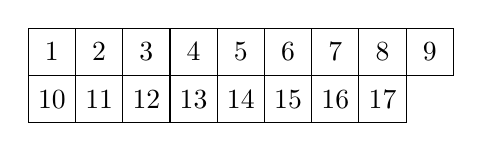
\begin{tikzpicture}
  \def\gridsize{9}
  \def\boxsize{0.6}
  \foreach \i in {1,...,\gridsize} {
  \pgfmathtruncatemacro\boxnumber{\i}
  \draw (\i*\boxsize, 0) rectangle ++(\boxsize, -\boxsize);
  \node at (\i*\boxsize+0.5*\boxsize, -0.5*\boxsize) {\boxnumber};
  }
  \def\gridsize{8}
  \foreach \i in {1,...,\gridsize} {
  \pgfmathtruncatemacro\boxnumber{\i+9}
  \draw (\i*\boxsize, -\boxsize) rectangle ++(\boxsize, -\boxsize);
  \node at (\i*\boxsize+0.5*\boxsize, -1.5*\boxsize) {\boxnumber};
  }
\end{tikzpicture}
